\documentclass{article}  % Define la clase del documento.

% Paquetes de idioma y codificación
\usepackage[utf8]{inputenc}
\usepackage[T1]{fontenc}
\usepackage[spanish]{babel}  % Ajusta el idioma del documento a español.
\usepackage{tabularx}  % Permite la creación de tablas con ancho ajustable.

% Paquete de geometría para configurar márgenes y tamaño de papel
\usepackage[letterpaper, margin=3cm]{geometry}

% Paquetes de tipografía
\usepackage{mathptmx}    % Usa Times New Roman como fuente.
\usepackage{microtype}   % Mejora la justificación del texto.

% Paquetes para manejo de colores y gráficos
\usepackage{xcolor}      % Define y utiliza colores.
\usepackage{graphicx}    % Permite la inserción de imágenes.
\usepackage{tikz}        % Creación de gráficos vectoriales.

% Configuración de enlaces y referencias cruzadas
\usepackage{hyperref}
\hypersetup{
    colorlinks   = true,
    linkcolor    = darkblue,
    citecolor    = black,
    filecolor    = blue,
    urlcolor     = blue
}

\usepackage{media9} % Permite la inserción de multimedia.

% Paquetes para la mejora visual de tablas y figuras
\usepackage{booktabs}    % Para tablas de alta calidad.
\usepackage{float}       % Controla la posición de figuras y tablas.

% Paquete para la personalización de códigos fuente
\usepackage{listings}
\lstset{
    literate=
    {á}{{\'a}}1 {é}{{\'e}}1 {í}{{\'i}}1 {ó}{{\'o}}1 {ú}{{\'u}}1
    {Á}{{\'A}}1 {É}{{\'E}}1 {Í}{{\'I}}1 {Ó}{{\'O}}1 {Ú}{{\'U}}1
    {ñ}{{\~n}}1 {Ñ}{{\~N}}1 {ü}{{\"u}}1 {Ü}{{\"U}}1,
    backgroundcolor=\color{backcolour},
    commentstyle=\color{codegreen},
    keywordstyle=\color{codepurple},
    numberstyle=\tiny\color{codegray},
    stringstyle=\color{red},
    basicstyle=\ttfamily\small,
    breakatwhitespace=false,
    breaklines=true,
    captionpos=b,
    keepspaces=true,
    numbers=left,
    numbersep=5pt,
    showspaces=false,
    showstringspaces=false,
    showtabs=false,
    tabsize=2,
    language=TeX,
    morecomment=[l]\#,
    frame=single,
    rulecolor=\color{black}
}

% Definición de colores al estilo Visual Studio Code
\definecolor{darkblue}{rgb}{0.0, 0.0, 0.55}  % Enlaces
\definecolor{codegreen}{rgb}{0.25, 0.49, 0.48}  % Comentarios
\definecolor{codegray}{rgb}{0.5, 0.5, 0.5}  % Números y anotaciones
\definecolor{codepurple}{rgb}{0.58, 0, 0.82}  % Palabras clave
\definecolor{backcolour}{rgb}{0.95, 0.95, 0.92}  % Fondo de código

% Configuraciones de párrafo y matemáticas
\usepackage{amsmath}
\usepackage{parskip}    % Espaciado entre párrafos.
\usepackage{ragged2e}   % Justificación mejorada.

% Configuración de secciones y encabezados
\usepackage{titlesec}
\titleclass{\part}{top} % Make part like a class
\titleformat{\part}[display]
  {\normalfont\huge\bfseries\centering}{\thepart}{40pt}{\Huge}
\titlespacing*{\part}{0pt}{-60pt}{10pt}
\titleformat{\part}
  {\normalfont\huge\bfseries}{}{0pt}{}

% Asegúrate de usar esto para mantener el estilo en las páginas de las partes
\titleformat{\part}[display]
  {\normalfont\huge\bfseries}{}{0pt}{}
  [\thispagestyle{fancy}] % Aplica el estilo fancy a las páginas de las partes

% Configuración de encabezados y pies de página personalizados
\usepackage{fancyhdr}
\pagestyle{fancy}
\fancyhf{}
\fancyhead[L]{\raisebox{0.20cm}{\textbf{Métodos Computacionales en Obras Civiles}}}
\fancyhead[R]{\raisebox{0.1cm}{
\includegraphics[width=0.25\linewidth]{LOGO_UNIVERSIDAD.jpg}}}
\fancyhead[C]{\rule{\textwidth}{0.6pt}}
\fancyfoot[C]{\rule{\textwidth}{0.6pt}}
\fancyfoot[R]{\raisebox{-1.5\baselineskip}{\thepage}}
\renewcommand{\headrulewidth}{0pt}
\renewcommand{\footrulewidth}{0pt}

% Configuración avanzada de geometría
\geometry{
  top=3.5cm, % Aumenta el espacio en la parte superior para subir el encabezado
  bottom=2.5cm,
  headheight=2.5cm % Aumenta la altura del encabezado si es necesario
}

% Configuracion de bibliografia
\usepackage{natbib}
\bibliographystyle{unsrtnat}  % Puedes cambiarlo por `unsrtnat`, `abbrvnat`, etc.
\usepackage{tabularx} 
\begin{document}
%----------------------------------------------------------------------------------------
% PORTADA
%----------------------------------------------------------------------------------------
\begin{titlepage}%Inicio de la carátula, solo modificar los datos necesarios
\newcommand{\HRule}{\rule{\linewidth}{0.5mm}} 
\center 
%----------------------------------------------------------------------------------------
%	ENCABEZADO
%----------------------------------------------------------------------------------------

\includegraphics[width=10cm]{LOGO_UNIVERSIDAD.jpg}\\ % Si esta plantilla se copio correctamente, va a llevar la imagen del logo de la facultad.OBS: Es necesario incluir el paquete: graphicx
\vspace{3cm}
%----------------------------------------------------------------------------------------
%	SECCION DEL TITULO
%----------------------------------------------------------------------------------------
\HRule \\[0.4cm]
{ \huge \bfseries Entrega 3, Proyecto 1}\\[0.4cm] % Titulo del documento
{ \huge \bfseries Metodos Computacionales en OOCC, IOC 4201}\\[0.4cm] % Titulo del documento
\HRule \\[1.5cm]
 \vspace{5cm}
%----------------------------------------------------------------------------------------
%	SECCION DEL AUTOR
%----------------------------------------------------------------------------------------
\begin{flushright}
    { \textbf{Profesor:}\\
    Patricio Moreno\\
    \vspace{0.2cm}
    \textbf{Ayudante:} \\
    Maximiliano Biasi\\
    \vspace{0.2cm}
    \textbf{Alumno:} \\
    Lukas Wolff Casanova\\
}
\end{flushright}
\vspace{1cm}
%----------------------------------------------------------------------------------------
%	SECCION DE LA FECHA
%----------------------------------------------------------------------------------------
{\large \textbf{\today}}\\[2cm] % El comando \today coloca la fecha del dia, y esto se actualiza con cada compilacion, en caso de querer tener una fecha estatica, reemplazar el \today por la fecha deseada
\end{titlepage}

\newpage
\thispagestyle{empty} % Deshabilita el número de página en la página del índice
\section*{Resumen}
Una ataguía es una estructura temporal utilizada para drenar zonas cubiertas de agua 
\citep{madanayaka2018}. En su diseño, es importante considerar factores como 
el caudal de infiltración, las presiones de poros y la estabilidad, donde la licuefacción
 es un fenómeno crítico. Este ocurre cuando las tensiones internas del suelo disminuyen,
  convirtiendo la mezcla de agua y sedimentos en un fluido, lo que puede comprometer 
  la estructura \citep{sumer2009}.
\\ \\
Existen diversos métodos para analizar redes de flujo: el cálculo teórico, 
el uso de grillas con diferencias finitas y los modelos a escala. El proyecto 
comparó estos procedimientos y concluyó que el de diferencias finitas es el más eficaz
 por su rapidez y precisión, aunque requiere un análisis previo. Por otra parte, el cálculo teórico es 
 lento y propenso a errores, mientras que los modelos a escala son útiles para calibrar 
 los resultados.
\\ \\
Finalmente, se utilizó el caudal de infiltración como parámetro de comparación entre los 
distintos modelos, observándose una diferencia de alrededor del 25\% entre el método
 teórico y el de diferencias finitas. Posteriormente, mediante el modelo a escala,
  se logró calibrar el código de diferencias finitas, lo que dio como resultado un error final del 
  7\%. En vista de todas las fuentes de error discutidas a lo largo del proyecto, 
  este error puede considerarse dentro de un rango esperado.

%----------------------------------------------------------------------------------------
%  INDICE
%----------------------------------------------------------------------------------------
\newpage
\thispagestyle{empty} % Deshabilita el número de página en la página del índice
\tableofcontents
\thispagestyle{plain} % Deshabilita el encabezado en la página del índice
\thispagestyle{empty} % Deshabilita el número de página en la página del índice

\thispagestyle{empty}
\listoffigures 
\thispagestyle{plain} % Deshabilita el encabezado en la página del índice %
\thispagestyle{empty}
\newpage
%----------------------------------------------------------------------------------------
%ACÁ EMPIEZA EL INFORME
\setcounter{page}{1}
%----------------------------------------------------------------------------------------

\part{Introducción}

Una ataguía es una estructura temporal utilizada para drenar zonas cubiertas de agua, lo que permite construir en terrenos que, de otra forma, serían inaccesibles \textbf{\cite{madanayaka2018}}. Hay varios factores importantes a considerar al momento de diseñar una ataguía, como el caudal de infiltración, las presiones de poros, la estabilidad de la estructura y, sobre todo, la licuefacción y su factor de seguridad (FS). Este último fenómeno ocurre cuando las presiones de poros alcanzan tal punto que las tensiones internas efectivas entre las partículas del suelo pierden efectividad, y, en consecuencia, la mezcla entre agua y sedimentos actúa como un fluido \textbf{\cite{sumer2009}}.
\\ \\
El presente proyecto tiene como objetivo el estudio y análisis de tres ataguías distintas, donde se busca evaluar sus características mediante cálculos manuales a través de Python, un solver mediante diferencias finitas y un modelo a escala. De esta manera, se busca analizar la efectividad de cada método de análisis, además de hacer una comparación directa entre los resultados obtenidos.
\\ \\
En los cálculos manuales, se utilizó la Ley de Darcy, además de las diferentes ecuaciones necesarias para determinar una red de flujo teórica. De esta forma, se calcularon parámetros como el caudal de infiltración y la presión de poros a lo largo de toda la estructura.
\\ \\
Posteriormente, se desarrolló un solver mediante diferencias finitas, el cual es un método numérico utilizado para calcular diferencias de potenciales en grillas 2D o 3D \textbf{\cite{zhang2005}}. De este modo, al determinar que el flujo va de un potencial mayor a uno menor, se pueden obtener las redes de flujo y, con ello, los distintos parámetros necesarios.
\\ \\
Finalmente, se realizó un modelo a escala, en el que se simuló la ataguía y una falla por licuefacción. Además, se buscó calibrar el modelo computacional en base a los datos obtenidos del modelo real, determinando así cuán efectivo es el cálculo numérico en comparación con la realidad.
\\ \\
El modelo base utilizado a lo largo del informe es el siguiente:

\begin{figure}[H]
    \centering
    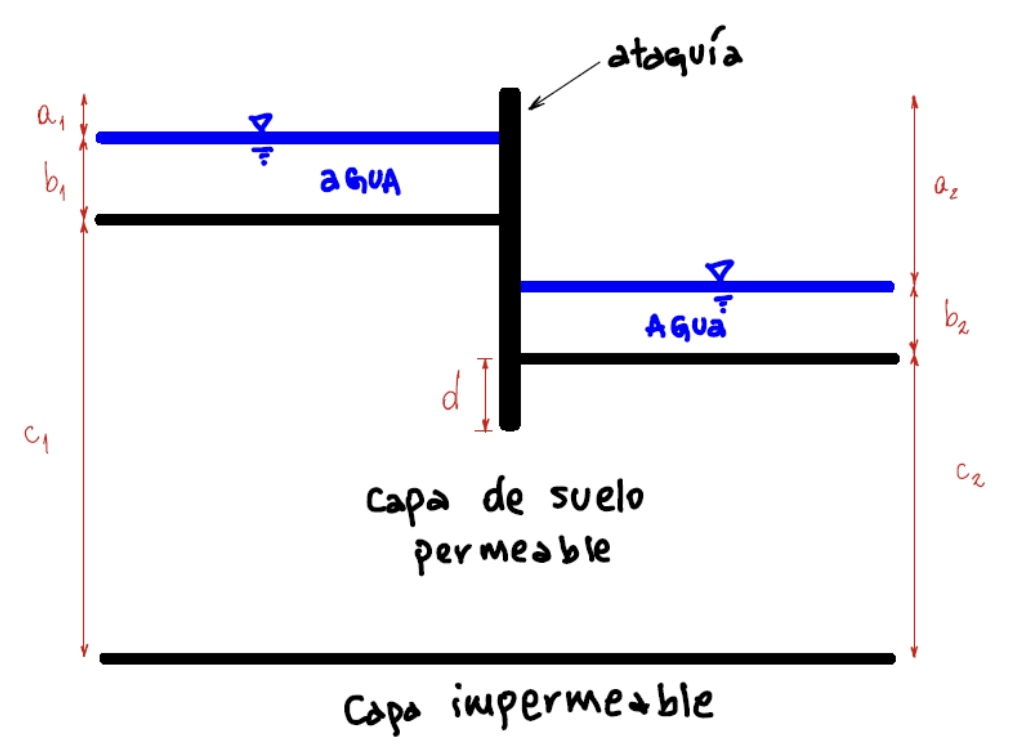
\includegraphics[width=0.45\textwidth]{FOTOS/modelo_base.png}
    \caption{Modelo Base}
    Fuente: Guía de Proyecto
    \label{fig:modelo_base}
\end{figure}

Las medidas para los distintos casos se encuentran en la tabla \textbf{\ref{tab:medidas}}.


\part{Calculos Manuales}

La presnete seccion tiene como objetivo modelar una ataguia utilizando redes de flujo y lineas equipotenciales graficadas $"$a mano $"$ a travez de python. De esta manera, se buscaran calcular factores como el caudal de infiltracion,
la presion de poros a lo largo de la ataguia, la estabilidad, falla por licuefaccion y factor de seguridad. Todos estas calculos fueron realizados mediante python, de esta manera, se pudo efectuar un analisis mas exausto y preciso en los distintos casos.

\section{Teoria}
\subsection{Líneas de Flujo}
Las líneas de flujo representan las trayectorias que siguen las partículas de agua al moverse a través de un medio poroso. En un diagrama de flujo, estas líneas son perpendiculares a las líneas equipotenciales y muestran la dirección del flujo subterráneo o de infiltración. En estructuras como las ataguías, las líneas de flujo se usan para predecir el comportamiento del agua alrededor y debajo de la estructura, ayudando a diseñar sistemas eficaces de control de agua. \textbf{\cite{structville}}

\subsection{Líneas Equipotenciales}
Las líneas equipotenciales representan ubicaciones con igual carga hidráulica, lo que significa que no hay diferencia de energía a lo largo de ellas. En problemas de flujo de agua subterránea, como los relacionados con las ataguías, estas líneas ayudan a visualizar la distribución de la energía potencial dentro del agua. Son fundamentales para determinar el caudal de agua y asegurar que esta no desestabilice estructuras como los diques o presas. \textbf{\cite{structville}}

\subsection{Caudal de infiltracion}

El caudal de infiltración es el flujo de agua que penetra a través del suelo, debido a la diferencia de presión entre el nivel de agua dentro y fuera de la ataguía en este caso. La tasa de infiltración esta condicionada por la permeabilidad del suelo y la diferencia de carga hidráulica. Para poder calcular el caudal de infiltración, se utiliza la fórmula (\ref{eq:caudal_infiltracion}). \textbf{\cite{stability_cofferdam_2024}}

\begin{equation}
    Q = k \cdot \frac{\Delta H}{N_{f}} \cdot N_{d}
    \label{eq:caudal_infiltracion}
\end{equation}

Donde:
\begin{itemize}
    \item $Q$ = Caudal de Infiltracion
    \item $k$ = Coeficiente de permeabilidad
    \item $\Delta H$ = Diferencia de carga hidraulica
    \item $N_{f}$ = Cantidad de canales de flujo
    \item $N_{d}$ = Cantidad de canales equipotenciales
\end{itemize}

\subsection{Presión de Poros}
La presión de poros es la fuerza que el agua ejerce dentro de los poros de un material como el suelo o la roca. Juega un papel crucial en la construcción con agua o alto nivel freático, ya que una presión de poros excesiva puede reducir el esfuerzo efectivo en el suelo, lo que podría ocasionar problemas como la licuefacción, donde el suelo pierde firmeza, o la formación de tuberías subterráneas. En las ataguías, la presión de poros es un factor clave, ya que afecta la estabilidad del terreno que rodea la estructura. Para poder calcular la presión de poros, se utiliza la siguiente formula. \textbf{\cite{jeas}}

\begin{equation}
    u = \gamma \cdot h
    \label{eq:presion_poros}
\end{equation}

Donde:
\begin{itemize}
    \item $u$ = Presión de Poros
    \item $\gamma$ = Peso Específico del Agua
    \item $h$ = Profundidad del agua
\end{itemize}


\subsection{Gradiente Hidráulico}
El gradiente hidráulico es el cambio de la carga hidráulica por unidad de distancia en la dirección del flujo. Es un factor crucial para determinar el flujo de agua a través de suelos. En el diseño de ataguías, el gradiente hidráulico ayuda a predecir problemas como la licuefacción, donde los gradientes elevados pueden erosionar el suelo y causar fallos estructurales. Este se calcula con la formula (\ref{eq:gradiente_hidraulico}). \textbf{\cite{budhu_soil_2010}}
\begin{equation}
    i = \frac{\Delta h}{\Delta L}
    \label{eq:gradiente_hidraulico}
\end{equation}
Donde:
\begin{itemize}
    \item $i$ = Gradiente Hidráulico
    \item $\Delta h$ = Cambio de carga hidráulica
    \item $\Delta L$ = Distancia en la dirección del flujo
\end{itemize}
\subsubsection{Licuefacción}
La licuefacción se genera cuando se excede el gradiente hidráulico crítico (\ref{eq:gradiente_critico}), lo que provoca que el suelo pierda su capacidad de soporte y se comporte como un líquido. En el diseño de ataguías, la licuefacción es un problema grave, ya que puede causar el colapso de la estructura y daños significativos a la infraestructura circundante. \textbf{\cite{budhu_soil_2010}}

\begin{equation}
    i_{critico} = \frac{\Delta h}{L_{min}}
    \label{eq:gradiente_critico}
\end{equation}

\subsection{Presión en una Ataguía}
La presión dentro y alrededor de una ataguía es resultado tanto del nivel de agua como de las condiciones del suelo. El diseño de una ataguía implica calcular la caída de carga potencial, la presión de poros y el gradiente hidráulico, lo que permite predecir si la estructura soportará las presiones del agua y del suelo que actúan sobre ella. Las redes de flujo se utilizan para evaluar estas presiones y estimar la infiltración de agua a través de la cimentación. \textbf{\cite{sivakugan2005}}






\part{Diferencias finitas}

Para mejorar la precisión de los resultados, se implementó un modelo de diferencias finitas aplicado a la matriz de potencial hidráulico. De esta manera, se pueden calcular las líneas de flujo, obteniendo así el caudal de infiltración. El objetivo principal es determinar la efectividad de este método frente a un proceso más simple, como el cálculo manual expuesto en la sección anterior.

\section{Teoría}

A continuación, se presentará la teoría utilizada para el cálculo en esta sección.

\subsection{Ley de Darcy}

La ley de Darcy se expresa como:

\begin{equation}
    q = k \cdot i \cdot A
\end{equation}

Lo cual es análogo a:

\begin{equation}
    v = k \cdot i
\end{equation}

Donde \(i\) es el gradiente hidráulico. Discretizando en el espacio, se obtiene lo siguiente:

\begin{equation}
    i = \frac{dh}{dl} = \frac{dh}{dx}; \frac{dh}{dy}; \frac{dh}{dz}
\end{equation}

Se define la entrada al sistema como:

\begin{figure}[H]
    \centering
    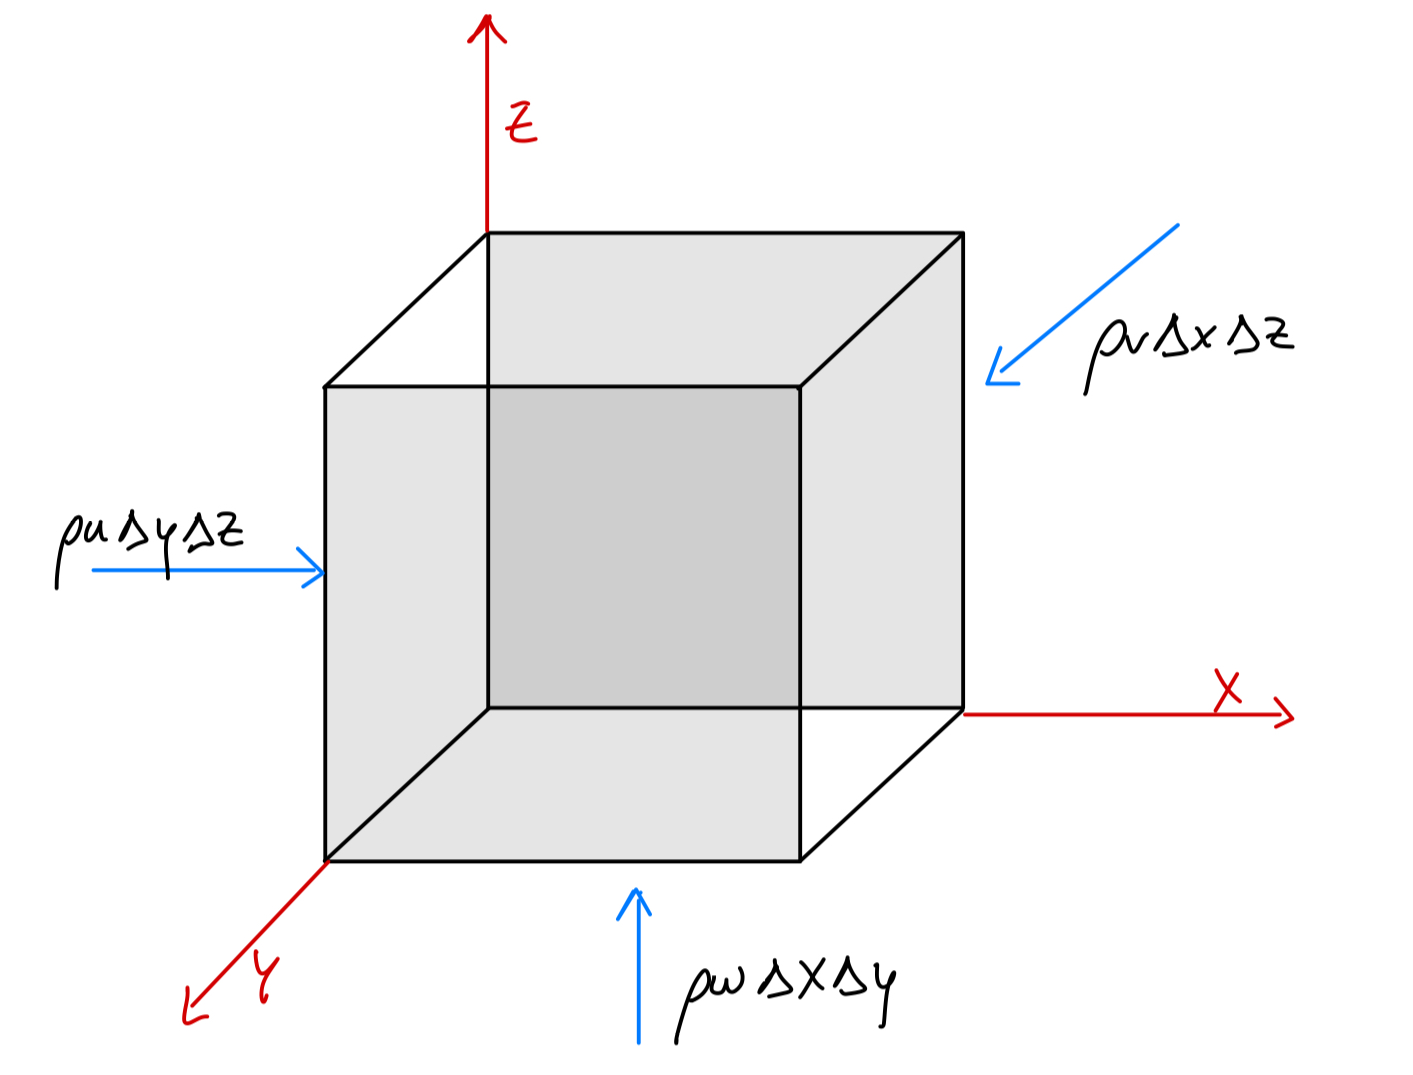
\includegraphics[width=0.5\textwidth]{FOTOS/in.jpg}
    \caption{Entrada al sistema}
    \text{Fuente: Elaboración propia}
    \label{fig:ley_darcy_in}
\end{figure}

La serie de Taylor expone que:

\begin{equation}
    f(x) = f(a) + \frac{df(a) \Delta X}{dx \cdot 1!} + ... + \frac{\Delta X^n}{n!} \cdot \frac{d^n f(a)}{dx^n}
\end{equation}

Por lo tanto, lo que sale del sistema es:

\begin{figure}[H]
    \centering
    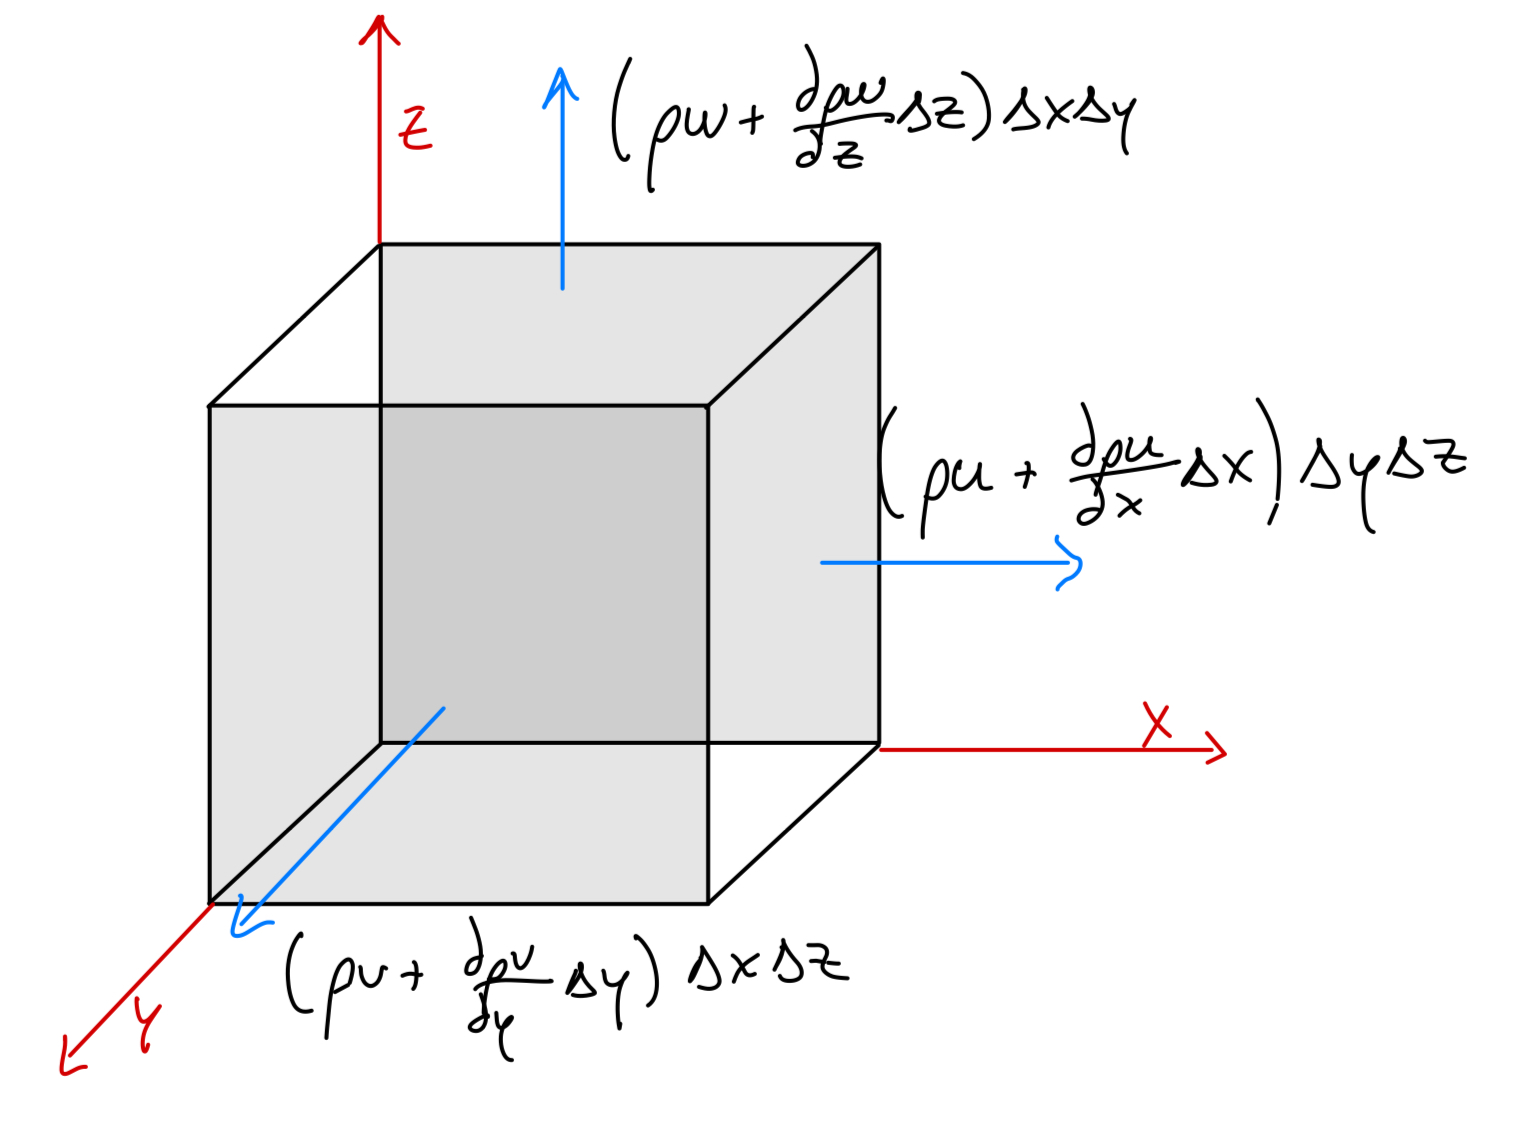
\includegraphics[width=0.5\textwidth]{FOTOS/out.jpg}
    \caption{Salida del sistema}
    \text{Fuente: Elaboración propia}
    \label{fig:ley_darcy_out}
\end{figure}

Luego, por conservación de masa:

\begin{equation}
    Q_{int} = Q_{out}
\end{equation}

De lo que se obtiene:

\begin{equation}
    \rho_u \Delta_y \Delta_z + \rho_v \Delta_x \Delta_z + \rho_w \Delta_x \Delta_y = (\rho_u + \frac{d\rho_u \Delta x}{dx})\Delta_y \Delta_z + (\rho_v + \frac{d\rho_v \Delta y}{dy})\Delta_x \Delta_z + (\rho_w + \frac{d\rho_w \Delta z}{dz})\Delta_x \Delta_y
\end{equation}

Simplificando:

\begin{equation}
    \Delta_x \Delta_y \Delta_z = Volumen
\end{equation}

Dado que el fluido es agua, que es incompresible, se tiene:

\begin{equation}
   -\rho(\frac{du}{dx}+ \frac{dv}{dy}+ \frac{dw}{dz}) = 0
\end{equation}

Lo cual es análogo a:

\begin{equation}
    -\rho \nabla \cdot \vec{v} = 0 = \nabla \cdot \vec{v}
\end{equation}

Por lo tanto, al reemplazar en la ley de Darcy, se obtiene:

\begin{equation}
    V_x = k_x\cdot \frac{dh}{dx}; V_y = k_y\cdot \frac{dh}{dy}; V_z = k_z\cdot \frac{dh}{dz}
\end{equation}

Incorporando la ecuación de continuidad, se obtiene:

\begin{equation}
    \nabla \cdot \vec{V} = \nabla \cdot (k \cdot \vec{i}) = 0
\end{equation}

Asumiendo un análisis en 2D, se tiene:

\begin{equation}
    \frac{d}{dx}(k_x \cdot \frac{dh}{dx}) + \frac{d}{dy}(k_y \cdot \frac{dh}{dy}) = 0
\end{equation}

Suponiendo que:

\begin{equation}
    k_x = k_y = k
\end{equation}

Se obtiene:

\begin{equation}
    k \nabla^2 h = 0
\end{equation}

De esta forma, podemos representar el laplaciano mediante diferencias finitas. \textbf{\cite{budhu_soil_2010}}

\subsection{Diferencias finitas}

\subsubsection{Diferencias hacia adelante}

\begin{equation}
    h(x + \Delta x) = h(x) + \frac{dh}{dx} \Delta x + ...
\end{equation}

\subsubsection{Diferencias hacia atrás}

\begin{equation}
    h(x - \Delta x) = h(x) - \frac{dh}{dx} \Delta x + ...
\end{equation}

\subsubsection{Diferencias centrales}

La suma de las diferencias hacia adelante y hacia atrás es:

\begin{equation}
    h(x + \Delta x) + h(x - \Delta x) = h(x) + \frac{d^2h}{dx^2}\frac{\Delta x}{2!} + ...(los pares)
\end{equation}

Donde la incógnita es $\frac{d^2h}{dx^2}$. Despejando, obtenemos:

\begin{equation}
    \frac{d^2h}{dx^2} = \frac{h(x + \Delta x) - 2h(x) + h(x - \Delta x)}{\Delta x^2}
\end{equation}

\begin{equation}
    \frac{dh}{dx} = \frac{h(x + \Delta x) - h(x)}{\Delta x}
\end{equation}

Esto se puede llevar a una grilla:

\begin{figure}[H]
    \centering
    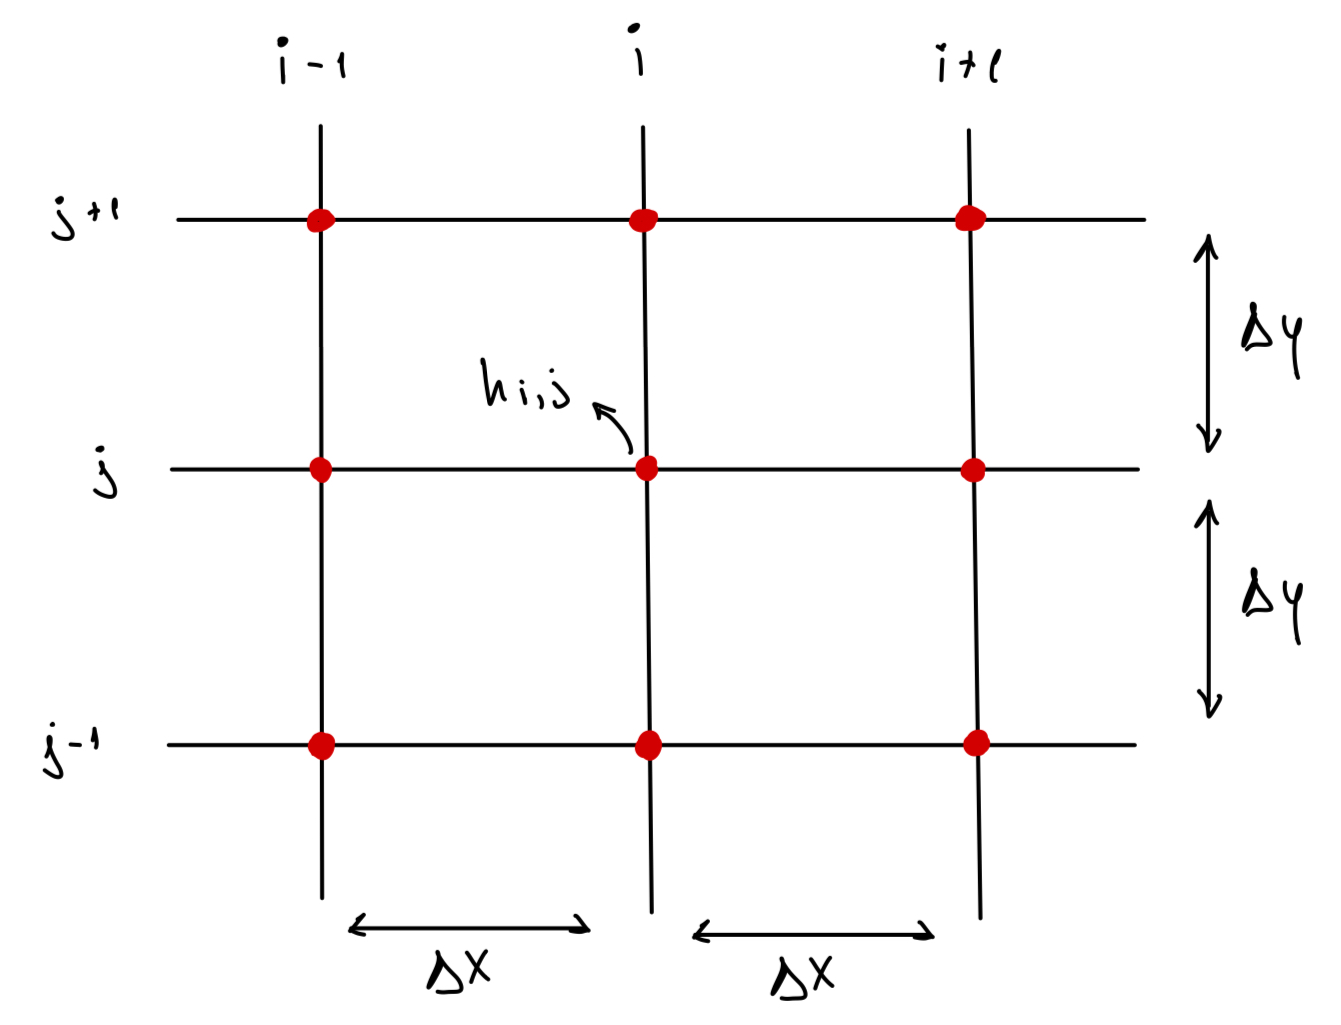
\includegraphics[width=0.5\textwidth]{FOTOS/grilla.jpg}
    \caption{Grilla}
    \text{Fuente: Elaboración propia}
\end{figure}

Donde se puede representar la ecuación de Laplace como:

\begin{equation}
    \frac{d^2h}{dx^2} = \frac{h_{i+1,j} + h_{i-1,j} - 2h_{i,j}}{\Delta x^2}
\end{equation}

\begin{equation}
    \frac{dh}{dx} = \frac{h_{+1,j} + h_{i+1,j}}{2\Delta x}
\end{equation}

Por lo tanto, podemos expresar la ley de Darcy con diferencias centrales, obteniendo:

\begin{equation}
    \frac{k}{\Delta^2}(h_{i+1,j} + h_{i-1,j} + h_{i,j+1} + h_{i,j-1} - 4h_{i,j}) = 0
\end{equation}

Donde se busca:

\begin{equation}
    h_{i,j} = \frac{1}{4}(h_{i+1,j} + h_{i-1,j} + h_{i,j+1} + h_{i,j-1})
\end{equation}

De esta forma, es posible obtener las variaciones en el potencial a partir de los datos conocidos en la grilla (condiciones de borde). \citep{budhu_soil_2010}

\subsection{Implementacion de diferencias finitas}

Al implementar este método, es necesario lograr que las paredes y la ataguía actúen como barreras impermeables, de manera que la variación de potencial sea cero en esos lugares. Además, se establecen dos condiciones de borde: el inicio y el fin del flujo hidráulico, donde se especifica el gradiente hidráulico en cada caso. De este modo, el flujo se desplaza desde un gradiente mayor hacia uno menor.


\newpage

\section{Resultados usando diferencias finitas}
Luego de implementar el método de diferencias finitas, se obtuvieron los siguientes resultados para los casos planteados en la sección anterior.
\subsection{Caso 1}

\begin{figure}[H]
    \centering
    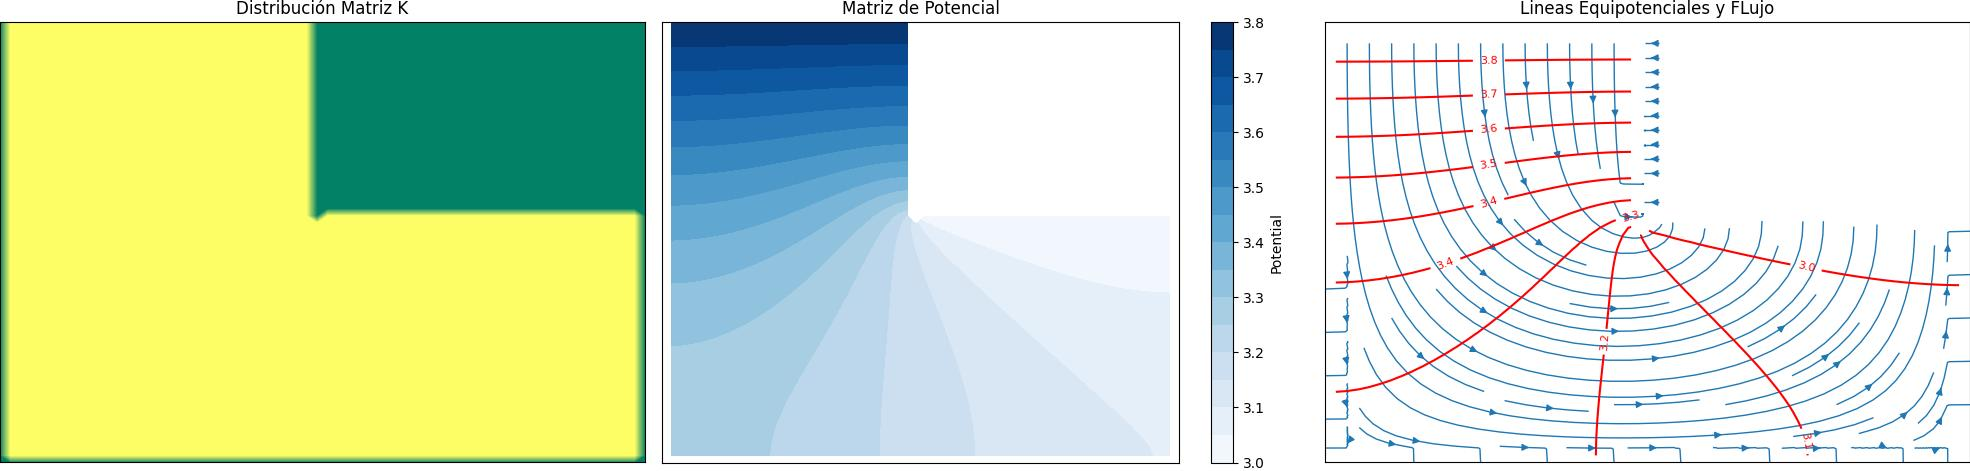
\includegraphics[width=\textwidth]{GRAFICOS/laplace_caso_1.jpg}
    \caption{Caso 1 Laplace}
    \text{Fuente: Elaboración propia}
    \label{fig:laplace_caso_1}
\end{figure}

Como aprecia en la figura \ref{fig:laplace_caso_1}, se cuanta con el mayor potencial hidráulico abajo de la ataguía, lo cual conlleva a un caudal de infiltración mayor que en los otros casos.

\subsection{Caso 2}

\begin{figure}[H]
    \centering
    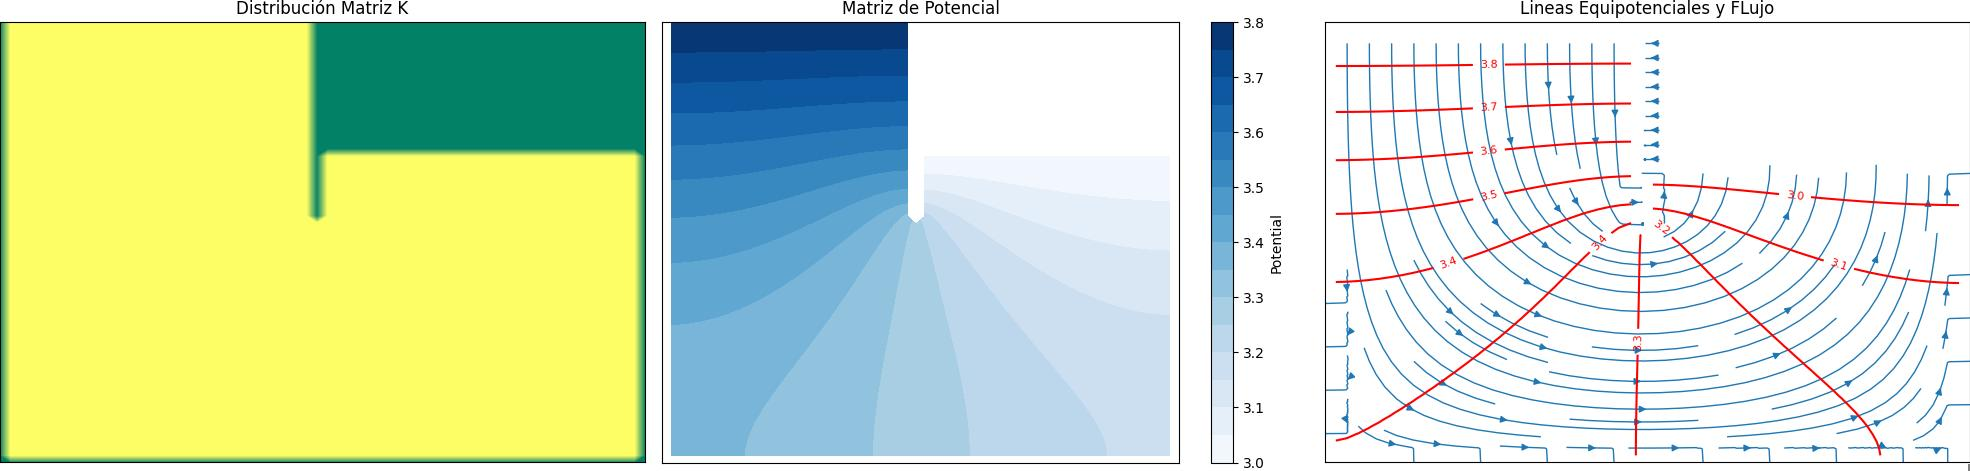
\includegraphics[width=\textwidth]{GRAFICOS/laplace_caso_2.jpg}
    \caption{Caso 2 Laplace}
    \text{Fuente: Elaboración propia}
    \label{fig:laplace_caso_2}
\end{figure}

Para el caso 2, se observa que se ocupó el mismo modelo, pero se modificaron las dimensiones y potenciales hidráulicos. Este cambio se puede apreciar en la distribución de la matriz \(K\) y en la matriz de potenciales. Además, en este caso, el potencial hidráulico abajo de la ataguía es menor.

\subsection{Caso 3}

\begin{figure}[H]
    \centering
    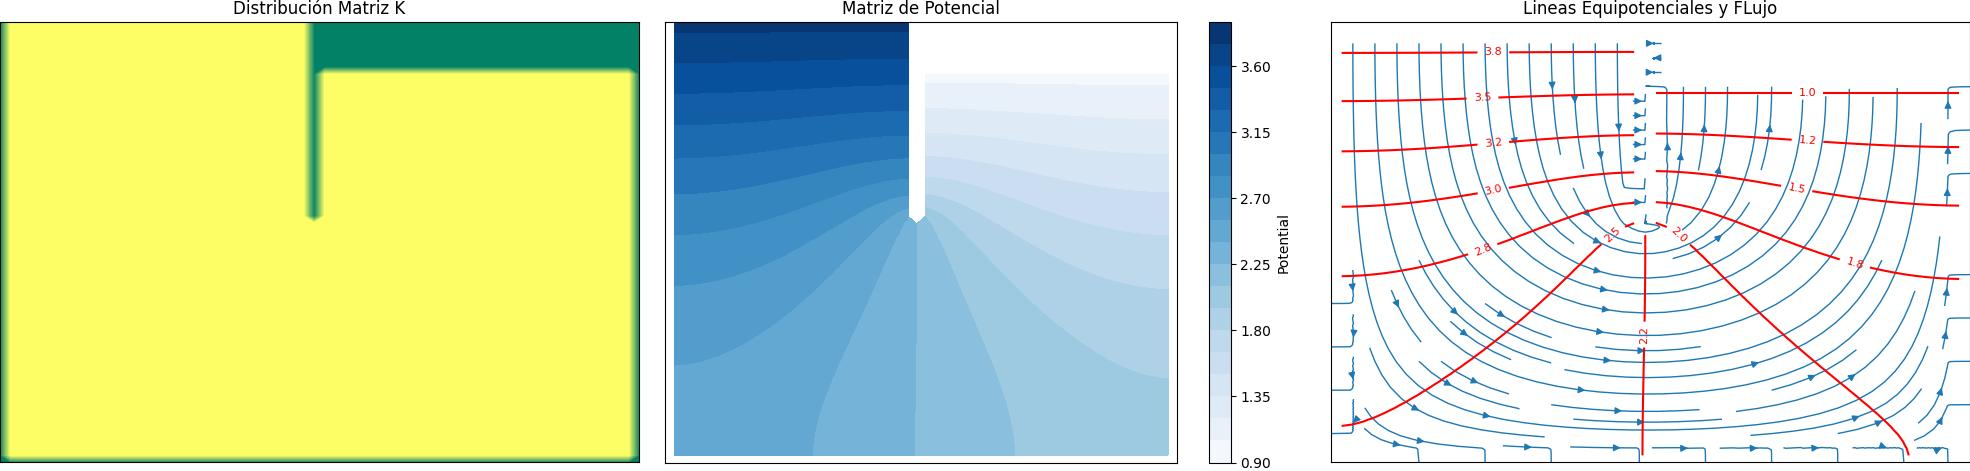
\includegraphics[width=\textwidth]{GRAFICOS/laplace_caso_3.jpg}
    \caption{Caso 3 Laplace}
    \text{Fuente: Elaboración propia}
    \label{fig:laplace_caso_3}
\end{figure}

Finalmente, en la figura \ref{fig:laplace_caso_3} se modificó la geometría del problema, la distribución de la matriz \(k\) y los potenciales hidráulicos. En este caso, el potencial hidráulico abajo de la ataguía es el menor de los tres casos, lo cual conlleva a un caudal de infiltración menor.

\section{Análisis de resultados}

\begin{table}[H]
    \centering
    \caption{Caudales obtenidos mediante análisis analítico y diferencias finitas}
    \vspace{0.5cm}
    \begin{tabular}{cccc}
        \hline
        \textbf{Caso} & \textbf{Caudal de Infiltración [$m/día$]} & \textbf{Caudal según Laplace [$m/día$]} & \textbf{Error [\%]} \\
        \hline
        1 & $0.97$ & $1.21$ & $24.7$ \\
        2 & $0.72$ & $0.99$ & $36.0$ \\
        3 & $0.57$ & $0.66$ & $15.8$ \\
        \hline
    \end{tabular}
    \text{Fuente: Elaboración propia}
    \label{tab:Diferencias1}
\end{table}

El método de diferencias finitas es una opción de cálculo más precisa que el método manual, ya que incorpora cada parte de la ataguía infinitesimalmente, calculando las presiones de manera más homogénea. Como resultado, se obtuvieron caudales menores y más representativos para cada caso, siendo los casos 1 y 2 caudales relativamente cercanos debido a que la altura de agua en ambos lados de la ataguía es la misma.
\\ \\
\textbf{Nota:} Se ocupa caudal por unidad lineal, ya que de esta manera se puede realizar una comparación mucho más objetiva para todo tipo de ataguía. 


\part{Modelo Escala}

\section{Resultados}

\subsection{Licuefaccion}

A continuacion se presenta un video de la falla observada por licuefaccion en la maqueta a escala.

\begin{center}
    \includemedia[
        width=0.5625\textwidth, % Relación de aspecto 9:16 (altura mayor que el ancho)
        height=\textwidth,
        activate=onclick,
        addresource=VIDEOS/licuefaccion.mp4,
        flashvars={
            source=VIDEOS/licuefaccion.mp4
        }
    ]{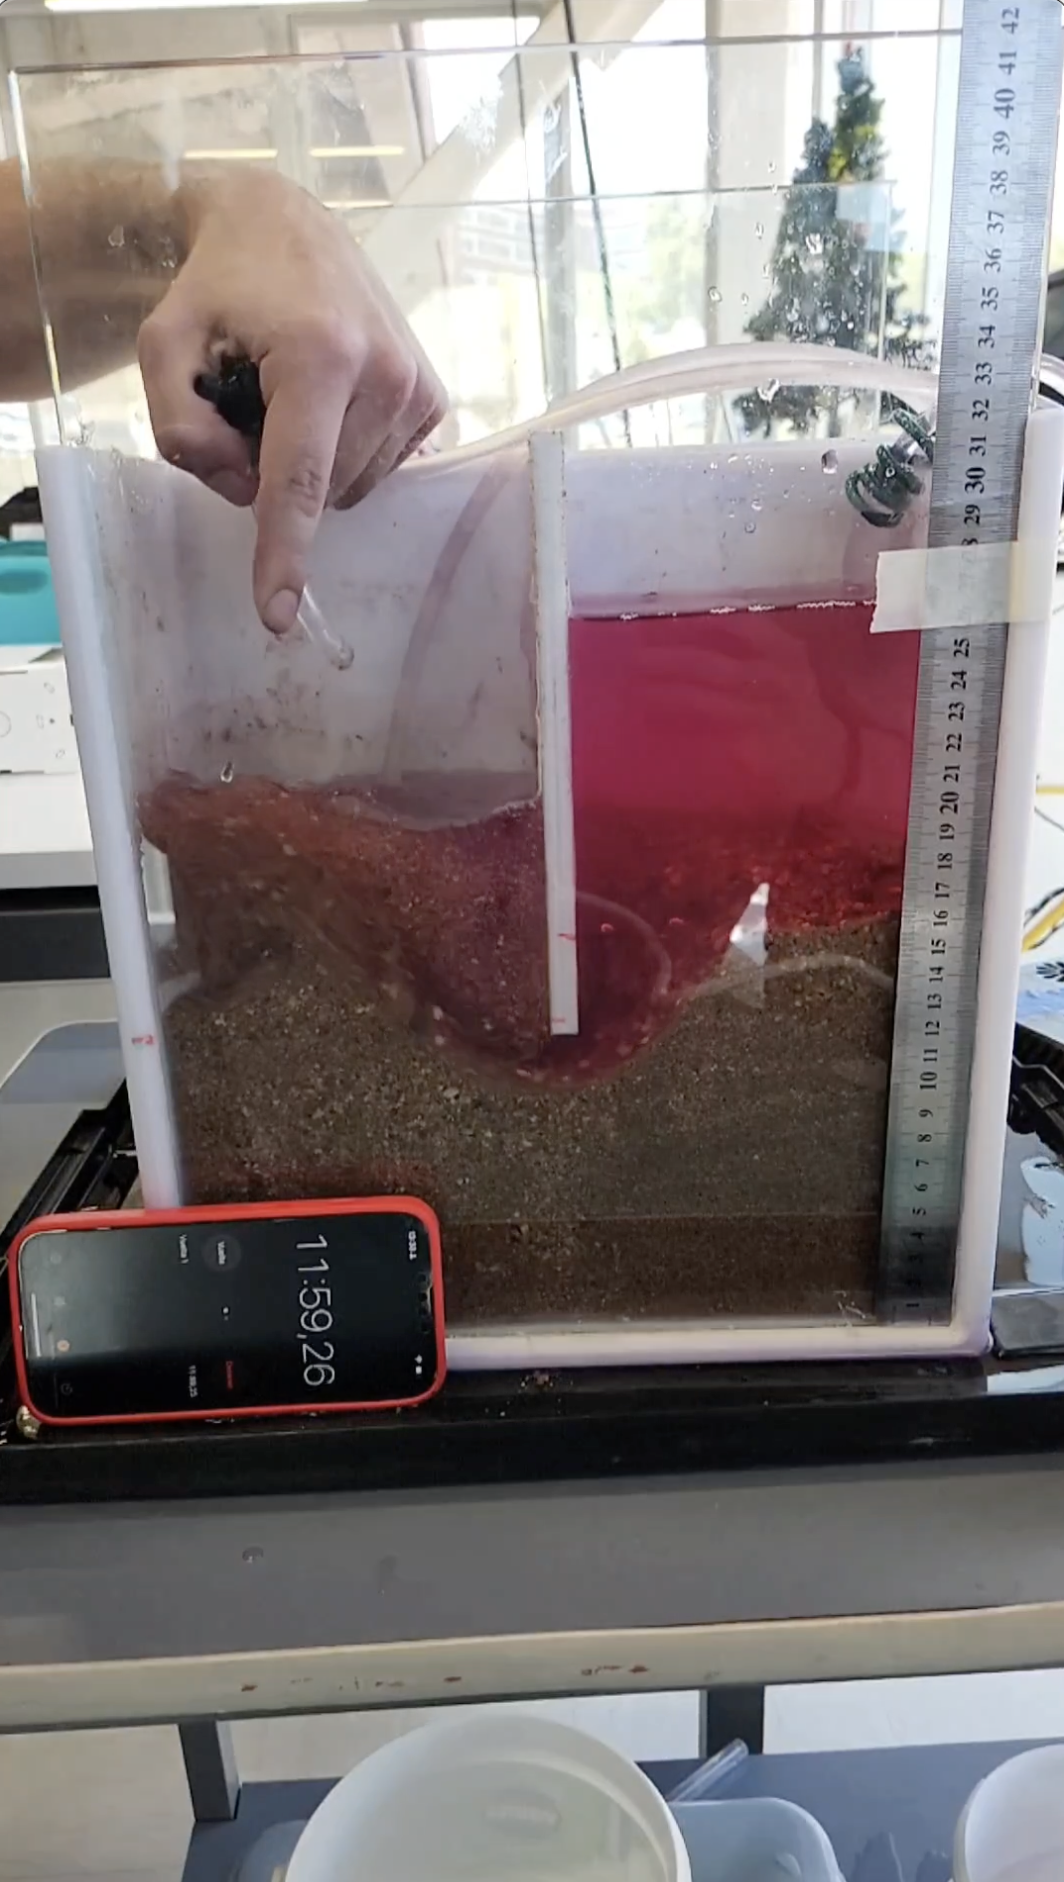
\includegraphics[width=\textwidth]{VIDEOS/miniatura_licuefaccion.png}}{VPlayer.swf}
\end{center}

\part{Conclucion}

%Párrafo 1. Resumen de lo que se hizo en el proyecto 
%Párrafo 2. Resumen de los modelos utilizados
%Párrafo 3 a 5 (aprox.) discusión de comparación de resultados entre las distintas aproximaciones (numérica y experimental) y resultados estadísticos. 
%Párrafo final. Crítica al modelo (supuestos, metodología, caso real vs caso simulado, etc.)

En conclucion, el presente proyecto tuvo como objetivo el estudio y análisis de 3 ataguías distintas, donde se buscó evaluar sus distintas características utilizando cálculos manuales a través de python, un solver mediante diferencias finitas y una maqueta a escala. 
De esta forma, se buscó analizar la efectividad de cada método de análisis, además de una comparación directa entre los resultados obtenidos. 
\\ \\
Analizando los 3 casos de estudio, se determino que el caso 3 es aque que presenta una mayor estabilidad, tanto por la licuefaccion, como por el momento que genera la presion de poros sobre la estructura misma (aun asi solo se esta analizando una seccion de toda la ataguia).
Se observo que el caudal de infiltracion esta directamente relacionado con el gradiente hidraulico, corrobroando la ley de Darcy. Finalmente, mediante un mapa de calor, se logro observar como se distribuyen las presiones de poros, ademas de la concentracion puntual que se da bajo
la ataguia cuando se produce la licuefaccion.
\\ \\
En cuanto a los calculos teoricos, se logro generar a travez de python un calculo correcto, donde posteriormente al comparar con las otras froams de resolucion, se puede concluir que la resolucion teorica es bastante fiable, aun asi, es dificil alcanzar una gran precision debido a la complejidad que esto conlleva. 
Las variaciones en los resultados, ademas del porcentaje de error estan dentro de un rango esperado.
\\ \\
Aplicando diferencias finitas se concluye que la precision de los resultados puede ser mucho mayor, aun asi, existe un punto donde aumentar la grilla deja de ser relevante, ya que el error se mantiene practicamente constante. Este modelo es mas complejo de aplicar, ya que rerquiere una comprencion de la teoria previamente, aun asi, es mucho mas eficiente y podria llegar a competir con los programas de pago actuales.
\\ \\
Comparando ambos metodos con el modelo a escala, se concluye que el calculo mediante diferencias finitas es mucho mas exacto, observando un error del 7\% con el modelo a escala realizado. Por otro lado, y comparando entre modelos, se observa un error en torno al 25\%, donde disminuir este dato es muy complejo por la parte torica, ya que requiere aumentar el numero de canales y lineas equipotenciales, lo cual aumenta la complejidad del calculo.
\\ \\
Finalmente el modelo a escala fue muy importante el la realizacion de esgte proyecto, ya que no solo permitio observar los distitnos fenomenos estudiados, sino que tambien pewrmitio calibrar y corroborar la informacion entregada por los modelos teoricos y computacionales. Aun asi, se critica el tipo de suelo utilizado, ya que este al tener una permeabilidad tan alta, genera que los valores obtenidos sean dificiles de controlar, donde ademas, es un suelo que dificilmente se presentara en una estructura como esta.
\\ \\


\section*{Anexos}

\begin{table}[H]
    \centering
    \begin{tabular}{|c|c|c|c|c|c|c|c|}
    \hline
    Caso & $a_1$ & $b_1$ & $c_1$ & $a_2$ & $b_2$ & $c_2$ & $d$ \\ \hline
    1    & 0.8   & 3.8   & 18.6  & 10.0  & 3.0   & 10.2  & 0.0 \\ \hline
    2    & 0.8   & 3.8   & 18.6  & 7.6   & 3.0   & 12.6  & 2.4  \\ \hline
    3    & 0.8   & 3.8   & 18.6  & 6.2   & 1.0   & 16.0  & 5.8  \\ \hline
    \end{tabular}
    \caption{Valores para casa caso [m]}
    \label{tab:medidas}
\end{table}
    

\newpage
\bibliography{referencias}  % Nombre del archivo .bib

\end{document}
